\documentclass[a4paper, 12pt, openany, oneside]{jsbook}

\usepackage[dvipdfmx]{graphicx}
\usepackage[dvipdfmx]{color}
\usepackage[dvipdfmx, bookmarks=true, setpagesize=false]{hyperref}
\usepackage{pxjahyper}
\usepackage[hang,small,bf]{caption}
\usepackage[subrefformat=parens]{subcaption}
\captionsetup{compatibility=false}

\usepackage{thesis}
\usepackage{here}
\usepackage{url}


\thesis{卒 業 論 文}
\title{
  \centering
    \scalebox{1.0}{視覚と行動の end-to-end 学習により経路追従行動を}\\
    \vspace{-0.3zh}
    \scalebox{1.0}{オンラインで模倣する手法の提案}\\
    \vspace{-0.3zh}
    \scalebox{1.0}{(目標方向による経路選択機能の追加)}\\
    \vspace{1zh}
    \scalebox{0.7}{A proposal for an online imitation method of path-tracking}\\
    \vspace{-0.8zh}
    \scalebox{0.7}{behavior by end-to-end learning of vision and action}\\
    \vspace{-0.8zh}
    \scalebox{0.7}{(Addition of path selection function by target direction)}\\
    \vspace{-7.0zh}
}
\setlength{\textwidth}{\fullwidth}
\setlength{\evensidemargin}{\oddsidemargin}

\date{\today}
\vspace{-15.0zh}
\teacher{林原 靖男 教授}
\vspace{-15.0zh}
\organization{千葉工業大学 先進工学部 未来ロボティクス学科}
\author{18C1096 春山 健太}
\vspace{-15zh}

\renewcommand{\baselinestretch}{1.2}
\begin{document}

%% Front Matter
\frontmatter{}
%
%!TEX root = ../thesis.tex
\bibliographystyle{plain}
\nocite{*}
\bibliography{main_bibliography}
%
% %!TEX root = ../thesis.tex
\chapter*{付録}
\addcontentsline{toc}{chapter}{付録}
%
学習結果から得られた重みで, 移動ロボットにドリブルを行わせた際の様子を動画に記録した. 以下にYoutubeに投稿した動画のURLを載せる.\\
%
\vspace{3.0zh}\\
%
実験1の結果\\
\url{https://youtu.be/aTAcS6ppBog} \\
\vspace{1.0zh}\\
実験2の結果\\
\url{https://youtu.be/GLhenu6ki8o} \\
\vspace{1.0zh}\\
実験3の結果\\
\url{https://youtu.be/9-IQF1eQCwk} \\
\vspace{1.0zh}\\
実験4の結果\\
\url{https://youtu.be/RQocHlh2Bxk} \\
\vspace{1.0zh}\\

%
%!TEX root = ../thesis.tex
\chapter*{謝辞}
\addcontentsline{toc}{chapter}{謝辞}

本研究を進めるにあたり,, 熱心にご指導していただいた林原靖男教授に深く感謝いたします.
また,研究の礎や研究へのアドバイスなどの様々な面で,指導,サポートしてくださった岡田眞也様,清岡優祐様には返しきれぬ恩をいただきました.
日々の生活の中で,議論や意見をしていただいたロボット設計制御研究室の皆様と
精神的に辛い際の支えであり,生活に潤いをくださった私の彼女へ感謝いたします.

最後に私を育てていただいた両親へ謝意を表します.


%
%% Main Matter
\mainmatter{}

\chapter{序論}
\section{背景}
近年,様々なセンサを用いた移動ロボットの自律移動に関する研究が盛んに行われており,
その中でカメラ画像を用いてロボットへ自律移動を行わせる研究も行われている.
%\index{うえだ@上田}
%例として,\cite{上田2015gihyo,ueda2015,上田2015jsai}がある.
Bojaskiら\cite{Nvidia}は
Fig. \ref{fig::nvidia}で示す方法で,人間のハンドル操作によるステアリングの角度の模倣学習を行い,
画像を用いて走行を行う方法を提案した.

\begin{figure}[h]
    \centering
    \includegraphics[width = 13cm]{./figs/EndtoEnd_Learning_for_Self-Driving_Cars.pdf}
    \caption{Training the neural network from \cite{Nvidia}}
    \label{fig::nvidia}
\end{figure}

\newpage
本研究室においても岡田ら\cite{okada}によってFig. \ref{fig::okada_sys}に示すシステム
LiDAR,オドメトリなどの入力としたルールべースの制御器の出力による自律走行を行い
その際にロボットから取得したカメラ画像を入力,ルールベース制御器の出力した角速度を目標出力として学習器の訓練を行い,
訓練後にはカメラ画像を入力を学習器へ入力し,その出力を用いて走行を行う
ルールベース制御器を用いてデータセット収集における労力の削減と経路へ戻る行動が学習可能な
Fig.\ref{fig::okada}で示すルールベース制御器の経路追従行動を模倣する手法が提案されている.
\begin{figure}[h]
    \centering
    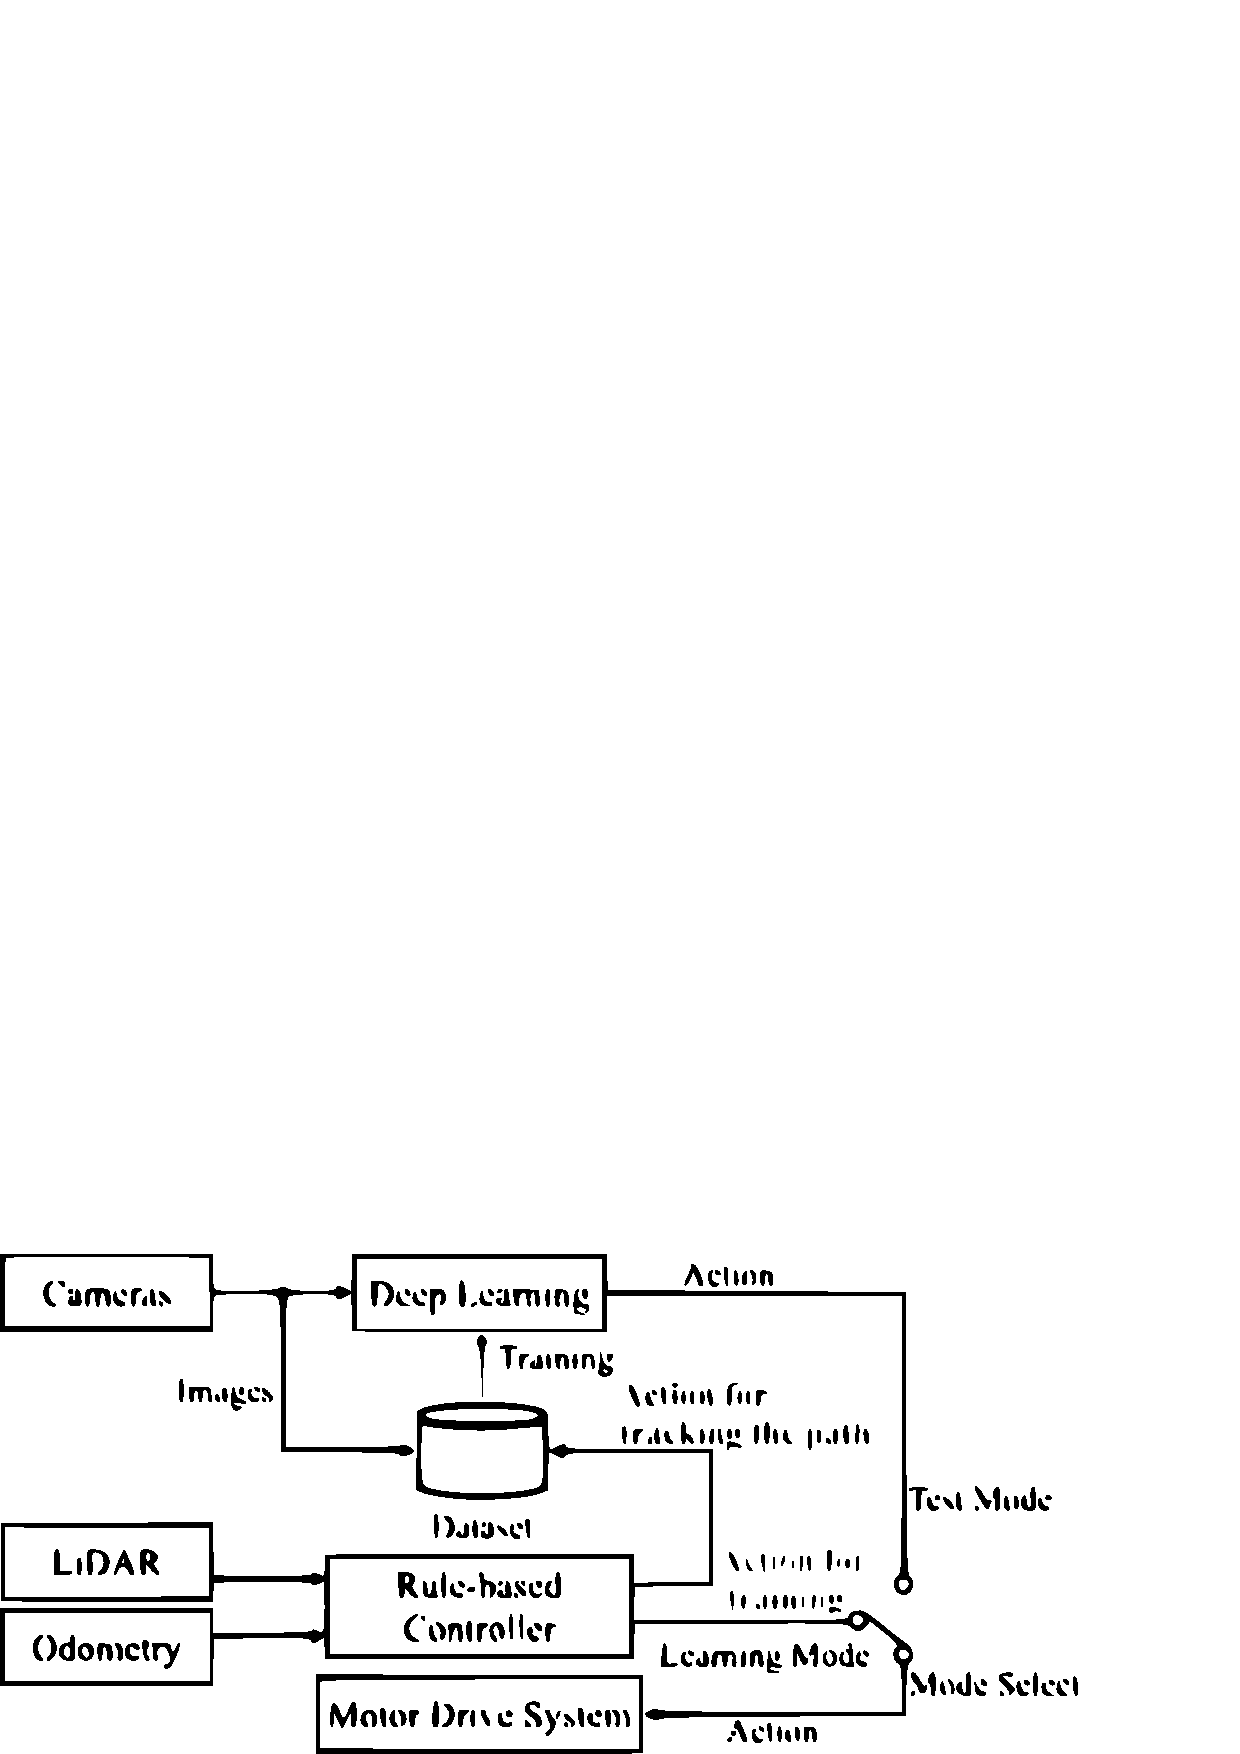
\includegraphics[width = 10cm]{./figs/okada_sys.png}
    \caption{Okada and others proposed method from \cite{okada}}
    \label{fig::okada_sys}
\end{figure}

\begin{figure}[h]
    \centering
    \includegraphics[width = 10cm]{./figs/okada.png}
    \caption{A robot that follows a path using vision based on the proposed method\cite{okada}}
    \label{fig::okada}
\end{figure}

\newpage
上記の研究により,カメラ画像用いてロボットが学習した経路を
周回可能であることが確認されている.


次に岡田ら\cite{okada}研究を一定の経路の周回以外への拡張について考える.
走行する経路内にFig. \ref{fig::bunki}のような分岐路が含まれる場合,
画像のみを入力としたネットワークでは,分岐路においてネットワークが2つの方向を出力してしまい,
左右に車体を向ける振動が発生してしまう事象がDean A. Pomerleauら\cite{pomeru}によって確認されている.
そのため赤と緑の矢印で示した直進と左折のようなルートを任意に切り替えを行うためには,
カメラ画像のみを入力とした場合「分岐路をどちらへ進むか」というルート選択を行うために
情報が必要だと考えられる.
 \vspace{4.0zh}
\begin{figure}[h]
    \centering
    \includegraphics[width = 8cm]{./figs/bunki.pdf}
    \caption{Cross road}
    \label{fig::bunki}
\end{figure}
\newpage

分岐路でルートをを選択をする情報として
人間の交差点などの目印に基づいて目的地まで移動する能力を,
島田らは分岐路などの目印(エッジ)とそのつながり(ノード)を表現する地図(トポロジカルマップ)
Fig. \ref{fig::topo}と
次の情報を持つエッジ
1) ID
2) Type(通路の特徴)
3) Edge(エッジの ID と相対角度)
トポロジカルマップより「道案内」同様に,「次の角まで」のような「条件」と「直進」などの「行動」
の組み合わせで作成した経路の情報(シナリオ)\ref{fig::sina}
を用いて表現した自律移動ロボットのNavigation手法を提案している.

\begin{figure}[H]
    \centering
    \includegraphics[width = 13cm]{./figs/topo.png}
    \caption{topo\cite{razikon}}
    \label{fig::topo}
\end{figure}
\begin{figure}[H]
    \centering
    \includegraphics[width = 13cm]{./figs/sina.png}
    \caption{sina\cite{razikon}}
    \label{fig::sina}
\end{figure}

そこで本研究では,島田らが提案した「シナリオ」から生成した
「直進」「左折」「右折」などの目標とする方向の情報(本研究では"目標方向"とする)
を\cite{okada}らが提案した手法において学習器の入力へ追加し,
学習器の出力を用いた走行で分岐路において特定のルート選択を行う
「カメラ画像と目標方向を用いたEnd-to-End学習によるシナリオを用いたNavigation手法」を提案する.
提案手法全体の流れをFig. \ref{fig::haikei_zentai}に示す.
\begin{figure}[H]
    \centering
    \includegraphics[width = 13cm]{./figs/haikei_zentai.pdf}
    \caption{hai}
    \label{fig::haikei_zentai}
\end{figure}

\newpage
カメラ画像と他の情報を用いて,自律移動を行う研究として
Felipeら\cite{razikon}はカメラ画像と操舵角と加速度の2次元の制御信号と,continue,left,straight,rightの4つのコマンドを入力としたネットワークを
用いてFig. \ref{fig::Conditional_Imitation_Learning}で示すように実環境と都市環境のシミュレータ上で学習器がコマンドに沿った行動が可能であることを
確認している.
\begin{figure}[H]
    \centering
    \includegraphics[width = 12cm]{./figs/End-to-end_Driving_via_Conditional_Imitation_Learning.pdf}
    \caption{End-to-end  Driving  via  Conditional  Imitation  Learning from \cite{razikon}}
    \label{fig::Conditional_Imitation_Learning}
\end{figure}

また,Seiyaら\cite{nagoya}はFig. \ref{fig::nagoyaabst}で示すように
カメラ画像と目標方向を入力,ステアリング制御信号を出力とするシステムを用いて,右および左に曲がる屋外の軌道を
追跡可能であることを確認している.

\begin{figure}[H]
    \centering
    \includegraphics[width = 9.8cm]{./figs/End-to-End_Navigation_with_Branch_Turning_Support_using_Convolutional_Neural_Network_abst.pdf}
    \caption{Overview of Seiya and others proposed method from \cite{nagoya}}
    \label{fig::nagoyaabst}
\end{figure}


\section{目的}
本研究では,岡田らと島田らの研究を拡張し,
カメラ画像と目標方向を用いたEnd-to-End学習
によるシナリオに基づいたNavigation手法を行う予備段階として
Fig. \ref{fig::haikei_abs}に赤枠で示した部分を対象とする,
\begin{figure}[H]
    \centering
    \includegraphics[width = 12cm]{./figs/haikei_abs.pdf}
    \caption{a}
    \label{fig::haikei_abs}
\end{figure}

カメラ画像と目標方向を入力とする学習器の出力を用いた走行において,
目標方向によって分岐路で任意のルートへ走行経路を変更することを目指す.
カメラ画像以外に分岐路での方向指示の情報を追加し,その情報を用いてルート選択が可能であるかの
検証を行う.


\section{論文構成}
1章では,本研究における背景,及び目的を述べた.
2章では,本研究で用いた深層学習の要素技術について述べる.
3章では,本研究で用いた手法と構築したシステムについて述べる.
4章では,構築したシステムを用いた実験を行う.
5章では,本研究の結論を述べる.

%要素技術
\chapter{要素技術}
本章では,本研究で用いた深層学習に関連した要素技術について述べる.

\section{Deep learning}
Deep learningは近年,自然言語処理など様々な分野で利用されている.
人間の脳におけるニューロンの構造を数理モデル(パーセプトロン)を用いて再現したニューラルネットワークを多層構造にすることで,
複雑なタスクの解決に必要な関数の表現力を高めたものである.
一般的な構造をFig. \ref{fig::network}示す.

\begin{figure}[h]
    \centering
    \includegraphics[width = 12cm]{./figs/net.pdf}
    \caption{Neual Network}
    \label{fig::network}
\end{figure}

\section{End-to-End学習}
End-to-Endとは「端から端まで」という,
Fig. \ref{fig::e2e}に示すように生データ(入力)から目的の結果(出力)を得るために必要な多段階の処理をNeusal Networkを用いて直接学習を行うものである.
例として,実世界における自動運転では人物や障害物などの物体認識,走行レーンの検出,経路計画,ステアリング制御
などの人間が設定した複数個のタスクを解く必要があるが,End-to-End学習では先程のタスクを人間が直接設定せずに
カメラ画像をニューラルネットワークに入力することで直接ステアリング操作を学習する.

\vspace{2.0zh}
\begin{figure}[h]
    \centering
    \includegraphics[width = 10cm]{./figs/e2e.pdf}
    \caption{Structure of End-to-End learning}
    \label{fig::e2e}
\end{figure}

\newpage
\section{Convolition Neual Network}
畳み込みニューラルネットワーク(convolutional neural network:CNN)は
画像認識や音声認識などの多次元の配列で表される複雑なデータを扱う処理へ用いられているニューラルネットワークである.
次のような特徴をもつ層で構成されている.

\begin{enumerate}
    \item 畳み込み層:入力データへフィルタ(カーネル)を用いて畳み込み演算を行うことで,特徴を抽出した特徴マップを取得する
    \item プーリング層:Maxプーリングなどの演算を用いて特徴マップのダウンサンプリングを行う
    \item 全結合層:畳み込み層,プーリング層で行った特徴を抽出したデータを一つのノードに
                      集約を行い,分類などの結果の出力を行う
\end{enumerate}


Krizhevskら\cite{Imagenet}はFig. \ref{fig::alex}で示すような3つの畳み込み層(convolutional layer),2つのプーリング層(pooling layer)
および 3 つの全結合層(fully connected layer)から構成したネットワークを用いて,
120万の高解像度画像を1,000の異なるクラスに分類をエラー率15.3\%で達成し,画像分類コンペティションであるILSVRC(ImageNet Large Scale Visual Recognition Competition)2012
で優勝をおさめた

\vspace{2.0zh}

\begin{figure}[h]
    \centering
    \includegraphics[width = 15cm]{./figs/alex.pdf}
    \caption{Alex net from \cite{Imagenet}}
    \label{fig::alex}
\end{figure}


% \include{purpose}MK
%提案手法
\chapter{提案手法}\label{chap:method}

\section{提案手法の概要}

1章の背景で述べたような分岐路において,ルートを選択する場合に
入力する情報としてカメラ画像のみでは「右と左のどちらに曲がる」という判断をするための情報が不足していると考えられる.
そこで,カメラ画像をもとにEnd-to-End学習で経路追従行動を行う
従来研究\cite{okada}で用いたシステムへカメラ画像以外にルートの選択に必要な情報として,「直進」「左折」「右折」の目標方向情報をコマンドを追加した,
提案手法の概要を以下に示す
学習フェーズ
テストフェーズ
本研究で対象とするロボットの構造,搭載するセンサを\ref{fig::turtlebot3_gazo}に示す.

\begin{figure}[H]
    \centering
    \includegraphics[width = 4cm]{./figs/turtlebot3_kame.pdf}
    \caption{turtlebot3 waffle}
    \label{fig::turtlebot3_gazo}
\end{figure}


% \begin{table}[ht]
%     \centering
%     \caption{Robot}
%       \begin{tabular}{c|cll}
%       \hline
%       tpye    & Differential-drive wheele                                                           \\ \hline
%       sensors & \begin{tabular}[c]{@{}l@{}}2D-LiDAR\\ Wheel Encoder\\ Monocular Camera\end{tabular} \\ \hline
%       \end{tabular}

    
%     \label{tb:hikaku}
   
%     \end{table}


\begin{figure}[H]
    \begin{tabular}{c}
      \begin{minipage}[t]{0.5\hsize}
        \centering
        \includegraphics[keepaspectratio, scale=0.4]{./figs/system_abs.pdf}
        \subcaption{Learning system}
        \label{exp29}
      \end{minipage}\\
      \begin{minipage}[t]{0.5\hsize}
        \centering
        \includegraphics[keepaspectratio, scale=0.4]{./figs/system_test_abs.pdf}
        \subcaption{Test system}
        \label{exp28}
      \end{minipage} \\
      \vspace{2.0zh}
    \end{tabular}
     \caption{Experiment 2 route}
     \label{fig::exp20}
  \end{figure}

\newpage
\section{システム}
本研究室のチームが行ってきたシステム\cite{okada}へ目標方向に対応したコマンドの生成機能とネットワーク構造の変更をすることでシステムを構築した.
「直進」「左折」「右折」の目標方向を要素数3,次元数1のint型の配列(One-Hot ベクトル)で表現し,方向と配列の対応をTable \ref{tb:comman}に示す.

本節では学習器の訓練を行う\ref{lerning}「学習フェーズ」,学習結果を用いて走行を行う\ref{test}「テストフェーズ」,
\ref{net}構築したネットワークの構造と\ref{seigyo}学習フェーズで用いる地図べースの制御器の4つに分けて述べる.
\vspace{2.0zh}
\begin{table}[h]
    \centering
    \caption{Command}
    \begin{tabular}{cccll}
    \cline{1-4}
    \multicolumn{1}{|c|}{Target Direction} & \multicolumn{1}{c|}{go straihgt}          & \multicolumn{1}{c|}{go left}          & \multicolumn{1}{c|}{go right}          &  \\ \cline{1-4}
    \multicolumn{1}{|c|}{data}  & \multicolumn{1}{c|}{{[} 100, 0, 0 {]}} & \multicolumn{1}{c|}{{[} 0, 100, 0 {]}} & \multicolumn{1}{l|}{{[} 0, 0, 100 {]}} &  \\ \cline{1-4}
                               &                                  &                                  &                                  &  \\
                               &                                  &                                  &                                  &  \\
    \multicolumn{1}{l}{}       &                                  &                                  &                                  & 
    \end{tabular}
    \vspace{-3.0zh}
    \label{tb:comman}
    \end{table}

\newpage
\section{地図ベースの制御器}
    \label{seigyo}
    学習フェーズで使用する地図ベースの制御器について,概要をFig. \ref{fig::navigation}に示す.
    センサからの観測情報を用いて局所的な障害物認識を行うlocal\_costmap,local\_costmapの結果を利用して局所的な経路計画を行うlocal\_planner.
    後述するmap\_serverから配信される,地図に対して全体のコスト計算を行うglobal\_costmap.
    その結果を利用して大域的な経路計画を行うglobal\_plannner.
    これらをレイヤーとして統合して行動計画とモータ指令を行う「move\_base」,Particle\_Filterによって自己位置推定を行う「amcl」,2つへ保持する地図の配信を行う
    「map\_server」などのパッケージを統合した自律移動用のメタパッケージである
    ROS Navigation\_stack\cite{navigation:online}へ目標地点(waypoint)とコマンドの生成機能をもつ「waypoint\_nav」を組み込んで使用している.
    \vspace{2.0zh}
    \begin{figure}[h]
        \centering
        \includegraphics[width = 12cm]{./figs/navigation.pdf}
        \caption{Map-based controller}
        \label{fig::navigation}
    \end{figure}


\newpage

\subsection{学習フェーズ}
\label{lerning}
学習器の訓練を行う学習フェーズで用いるシステムをFig. \ref{fig::learningsystem}示す.
学習は下記の一連の流れを1stepとして,設定したstep数行う.
\begin{enumerate}
    \item LiDARとオドメトリを入力とする地図ベースの制御器の出力を用いて自律走行を行う
    \item 地図ベースの制御器の出力からヨー方向の角速度とコマンド,機体に取り付けたカメラからRGB画像を取得し,訓練データへ加える
    \item 訓練データを 入力:カメラ画像,コマンド 目標出力:角速度 として学習器へ渡す
    \item 学習器の出力を記録.
  \end{enumerate}
画像の取得には従来研究\cite{okada}にならって,機体の中央, 中央に対して左,右に傾けて取り付けた3つのカメラを用いる.
また分岐路以外では,1つのコマンド(例として「直進」)を出力し続けた場合にデータセットへ偏りが生じる可能性が考えられるため,
ランダムなコマンドの出力を用いる.
コマンドの生成方法は\ref{seigyo}で述べるwaypointを用いて,目標方向に対応したコマンドを生成する.

\begin{figure}[H]
    \centering
    \includegraphics[width = 12cm]{./figs/system_learning.pdf}
    \caption{Learning system }
    \label{fig::learningsystem}
\end{figure}


\newpage
\subsection{テストフェーズ}
\label{test}
設定したstep数に達した場合に,Fig. \ref{fig::testsystem}に示すように
地図ベースの制御器の出力による動作から,中央のカメラ画像とコマンドを入力とした
学習器の出力による動作へ切り替えて走行を行う.
テスト時のコマンドの生成(方向の指示)はJoy\_stickコントローラのボタンを用いて行う.
テストフェーズにおける手順を下記に示す.
\begin{enumerate}
    \item 機体に取り付けた中央のカメラからRGB画像,Joy\_stickコントローラよりコマンドのデータを取得
    \item 取得したデータ(カメラ画像,コマンド)を学習器へ入力
    \item 学習器の出力である角速度をモータへ与える
  \end{enumerate}


\begin{figure}[h]
    \centering
    \includegraphics[width = 12cm]{./figs/system_test.pdf}
    \caption{Test system}
    \label{fig::testsystem}
\end{figure}

\newpage
\section{ネットワーク構造}
\label{net}
今回のシステムで用いたネットワークをFig. \ref{fig::methodnetwork}に示す.
また,ハイパーパラメータについてTable \ref{tb::param}に示す.
64×48のRGB画像を入力とする入力層1,畳込み層3,全結合層2層を持つ6層のCNNと,CNNの出力とコマンドを入力する入力層1,
全結合層2.出力層1の全10層の構造になっている.
出力はヨー方向の角速度を連続値である.

\begin{figure}[h]
    \centering
    \includegraphics[width = 13cm]{./figs/network.pdf}
    \caption{Method network}
    \label{fig::methodnetwork}
\end{figure}
% \vspace{-1.0zh}
\begin{table}[h]
    \centering
    \caption{Parameters of deep learning}
    \begin{tabular}{|c|c|c|c|}
    \hline
    Input Data    & Image (64x48 pixels, RGB channels) , Command                                              \\ \hline
    Optimizer     & Adam ($alpha = 0.001, beta1 = 0.9, beta2 = 0.999, eps = 1e^{-1}$ )  \\ \hline
    Loss Function & Softmax-cross-entropy                                                            \\ \hline
    Output Data   & Angular velocity                                              \\ \hline
    \end{tabular}
    \label{tb::param}
    \end{table}
\newpage





%実験
\chapter{実験}
\section{実験環境}
実験はシミュレータ上で行い,
シミュレータ環境としてオープンソースの3DロボットシミュレータGazebo\cite{gazebo:online}を用いる.
使用機体についてはturtlebot3\_waffle\cite{turtlebot3:online}へカメラを3つ追加したモデル\ref{fig::turtlebot3}を使用する.

\begin{figure}[H]
    \centering
    \includegraphics[width = 10cm]{./figs/3_camera.png}
    \caption{Turtlebot3 waffle add 3 cameras}
    \label{fig::turtlebot3}
\end{figure}

\section{実験方法}

実験における手順を下記に示す
\begin{enumerate}
  \item 学習フェーズを行い,学習器の訓練(経路の学習)行う 
        
  (制御:地図べースの制御器の出力)
  \item 設定したstep数を学習後,訓練フェーズへ移行 
  
  (制御:学習器の出力)
  \item コース内に設定した地点において目標方向のコマンドを入力,挙動を確認
\end{enumerate}
実験はコース内に設定した地点ごとにコマンドの入力による挙動の確認を5回ずつ行う. 
  また,用いるコースは実験ごとに異なるものを用いる.

\section{成功失敗条件}
実験の評価条件を下記のように定義する

成功:分岐路において壁に衝突せず,コマンドに対応したコースを選択

失敗:コマンドとは異なったコースを選択する,分岐路において壁に衝突

\newpage
\section{実験1 十字路}
\subsection{実験目的}
提案手法を用いて,分岐路においてコマンドによってルートの変更が可能であるかの検証を行う.
\subsection{実験環境}
学習step数:4000[step]
Fig. \ref{fig::zyuzi}に示す道幅が2.5m幅の十字路の環境を用いる.
\begin{figure}[ht]
    \centering
    \includegraphics[width = 10cm]{./figs/zyuuziyoko.png}
    \caption{Course of experiment1}
    \label{fig::zyuzi}
\end{figure}

\newpage
\subsection{学習フェーズでの経路}
学習時の経路についてFig. \ref{fig::exp1route}に示す
Fig内の緑で示す箇所が初期位置,赤で示す円が目標地点である
目標地点を1,2,3の順で走行し,到達後初期値点へロボットの位置,姿勢をリセットする.

\begin{figure}[ht]
    \centering
    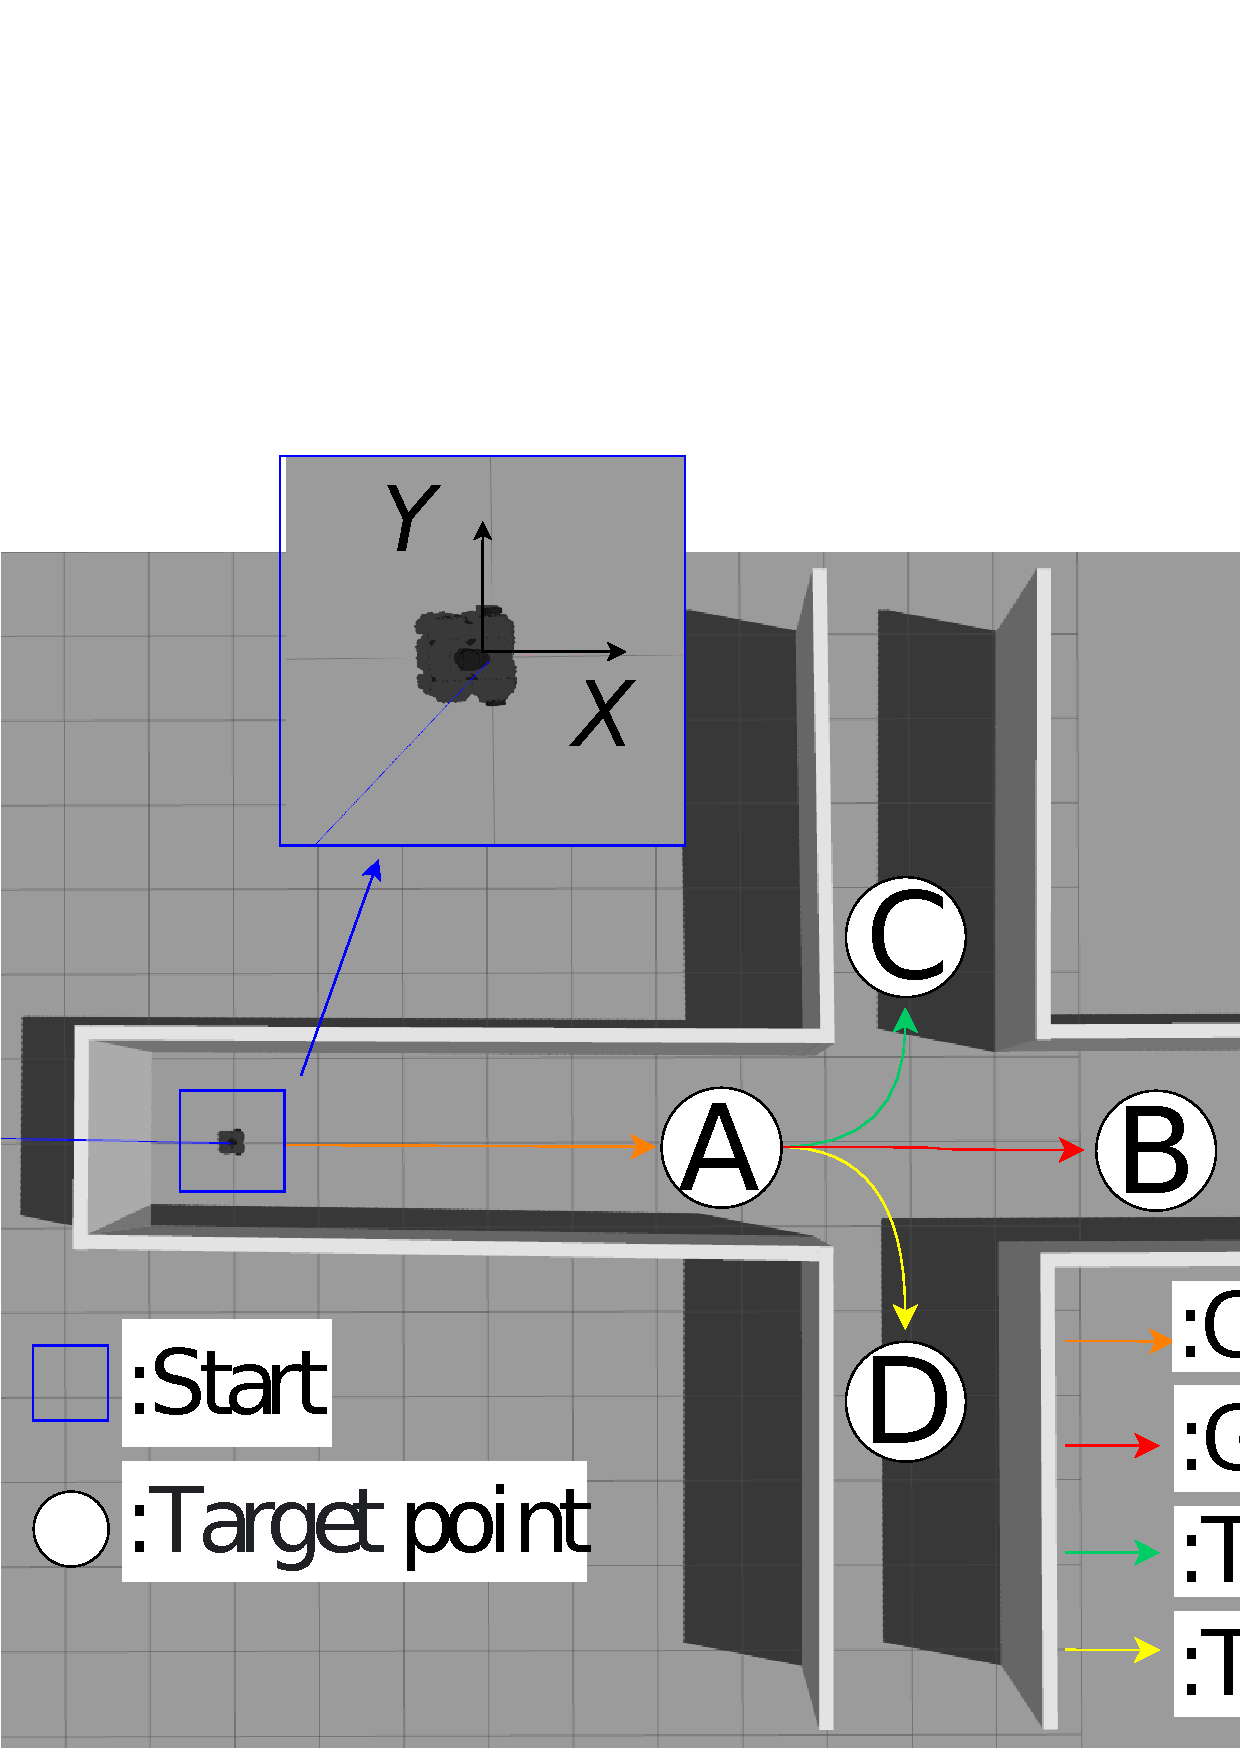
\includegraphics[width = 10cm]{./figs/zyuziroute.pdf}
    \caption{Route of experiment 1}
    \label{fig::exp1route}
\end{figure}

\subsection{評価}

Fig. \ref{fig::exp1route}で青で示した地点において,
コマンドを入力を行った結果をTable. \ref{tb::exp1suc}に示す.
\begin{table}[H]
  \centering
  \caption{Number of successes experiment 1 point}
  \begin{tabular}{|c|c|}
  \hline
  Point & Number of successes \\ \hline
  1     & /5                  \\ \hline
  2     & /5                  \\ \hline
  3     & /5                  \\ \hline
  \end{tabular}
  
  \label{tb::exp1suc}
  \end{table}

\newpage
\section{実験2 八の字}
\subsection{実験目的}
実験1で用いた局所的な環境を更に複雑な環境へ拡張し,
提案手法を用いて,分岐路においてコマンドによってルートの変更が可能であるかさらなる検証を行う.
\subsection{実験環境}
学習step数:60000step
Fig. \ref{fig::hatinozi}に示す道幅が2.5m幅の八の字型の環境用いる.
\begin{figure}[h]
    \centering
    \includegraphics[width = 10cm]{./figs/coli.png}
    \caption{Experiment2 Course}
    \label{fig::hatinozi}
\end{figure}

\newpage
\subsection{学習フェーズでの経路}
学習時の経路についてFig. \ref{fig::exp2route}に示す.
Route 1-6のルートを繰り返し周回する.

\begin{figure}[H]
    \begin{tabular}{cc}
      \begin{minipage}[t]{0.5\hsize}
        \centering
        \includegraphics[keepaspectratio, scale=0.4]{./figs/8nozi_1.pdf}
        \subcaption{Route 1}
        \label{exp2route1}
      \end{minipage} 
      \begin{minipage}[t]{0.5\hsize}
        \centering
        \includegraphics[keepaspectratio, scale=0.4]{./figs/8nozi_2.pdf}
        \subcaption{Route 2}
        \label{exp2route2}
      \end{minipage} \\
      \vspace{2.0zh}
      \begin{minipage}[t]{0.5\hsize}
        \centering
        \includegraphics[keepaspectratio, scale=0.4]{./figs/8nozi_3.pdf}
        \subcaption{Route 3}
        \label{exp2route3}
      \end{minipage} 
      \begin{minipage}[t]{0.5\hsize}
        \centering
        \includegraphics[keepaspectratio, scale=0.4]{./figs/8nozi_4.pdf}
        \subcaption{Route 4}
        \label{exp2route4}
      \end{minipage}\\

      \begin{minipage}[t]{0.5\hsize}
        \centering
        \includegraphics[keepaspectratio, scale=0.4]{./figs/8nozi_5.pdf}
        \subcaption{Route 5}
        \label{exp2route5}
      \end{minipage} 
      \begin{minipage}[t]{0.5\hsize}
        \centering
        \includegraphics[keepaspectratio, scale=0.4]{./figs/8nozi_6.pdf}
        \subcaption{Route 6}
        \label{exp2route6}
      \end{minipage} 
    \end{tabular}
     \caption{Experiment 2 route}
     \label{fig::exp2route}
  \end{figure}
  
\newpage
\subsection{評価}
コース内の各地点へFig. \ref{fig::bunkiban}で示すように番号をふり,地点ごとの成功回数を
Table. \ref{tb::exp2suc}に示す.
\begin{figure}[h]
  \centering
  \includegraphics[width = 10cm]{./figs/bunkiban.pdf}
  \caption{Experiment 2 point number}
  \label{fig::bunkiban}
\end{figure}


\begin{table}[H]
  \centering
  \caption{Number of successes Experiment2 point}
  \begin{tabular}{|c|c|}
  \hline
  Point & Number of successes \\ \hline
  1     & /5                  \\ \hline
  2     & /5                  \\ \hline
  3     & /5                  \\ \hline
  4     & /5                  \\ \hline
  5     & /5                  \\ \hline
  6     & /5                  \\ \hline
  7     & /5                  \\ \hline
  8     & /5                  \\ \hline
  9     & /5                  \\ \hline
  10    & /5                  \\ \hline
  11    & /5                  \\ \hline
  12    & /5                  \\ \hline
  \end{tabular}
  
  \label{tb::exp2suc}
  \end{table}
  
% \newpage
% \section{実験3 千葉工業大学津田沼校舎2号館3階}
% \subsection{実験環境}
% 〜に示す道幅が2.5m幅の八の字型の環境用いる.
% \subsection{実験目的}
% 実環境に近い環境で実験を行う
% \subsection{学習フェーズでの経路}
% 蟹
%結論
\chapter{結論}

本研究では,岡田ら\cite{okada}らのカメラ画像を用いて経路追従行動を行う手法を拡張し,
カメラ画像とコマンドを用いた分岐路で任意のルートを選択する手法を提案し,シミュレータを用いて検証を行った.

目標方向のデータセットに偏りが原因であると考えられる.
今後は偏りの解消法及びシステムへシナリオを組み込む
あとはまとまり次第書きます
%謝辞
% \chapter*{謝辞}\addcontentsline{toc}{chapter}{謝辞}

熱心に指導されてくださった林原靖男教授
また先行研究や研究へのアドバイスなどの様々な面で,指導,サポートしてくださった
岡田眞也先輩,清岡優祐先輩.
私生活で精神面でのサポートをしていただいた蟹さん

母なる大地に感謝

%% Appendix
% \appendix{}
% %!TEX root = ../thesis.tex
\chapter*{付録}
\addcontentsline{toc}{chapter}{付録}
%
学習結果から得られた重みで, 移動ロボットにドリブルを行わせた際の様子を動画に記録した. 以下にYoutubeに投稿した動画のURLを載せる.\\
%
\vspace{3.0zh}\\
%
実験1の結果\\
\url{https://youtu.be/aTAcS6ppBog} \\
\vspace{1.0zh}\\
実験2の結果\\
\url{https://youtu.be/GLhenu6ki8o} \\
\vspace{1.0zh}\\
実験3の結果\\
\url{https://youtu.be/9-IQF1eQCwk} \\
\vspace{1.0zh}\\
実験4の結果\\
\url{https://youtu.be/RQocHlh2Bxk} \\
\vspace{1.0zh}\\

%
%% Back Matter
\backmatter{}
%
%!TEX root = ../thesis.tex
\bibliographystyle{plain}
\nocite{*}
\bibliography{main_bibliography}
%
% %!TEX root = ../thesis.tex
\chapter*{付録}
\addcontentsline{toc}{chapter}{付録}
%
学習結果から得られた重みで, 移動ロボットにドリブルを行わせた際の様子を動画に記録した. 以下にYoutubeに投稿した動画のURLを載せる.\\
%
\vspace{3.0zh}\\
%
実験1の結果\\
\url{https://youtu.be/aTAcS6ppBog} \\
\vspace{1.0zh}\\
実験2の結果\\
\url{https://youtu.be/GLhenu6ki8o} \\
\vspace{1.0zh}\\
実験3の結果\\
\url{https://youtu.be/9-IQF1eQCwk} \\
\vspace{1.0zh}\\
実験4の結果\\
\url{https://youtu.be/RQocHlh2Bxk} \\
\vspace{1.0zh}\\

%
%!TEX root = ../thesis.tex
\chapter*{謝辞}
\addcontentsline{toc}{chapter}{謝辞}

本研究を進めるにあたり,, 熱心にご指導していただいた林原靖男教授に深く感謝いたします.
また,研究の礎や研究へのアドバイスなどの様々な面で,指導,サポートしてくださった岡田眞也様,清岡優祐様には返しきれぬ恩をいただきました.
日々の生活の中で,議論や意見をしていただいたロボット設計制御研究室の皆様と
精神的に辛い際の支えであり,生活に潤いをくださった私の彼女へ感謝いたします.

最後に私を育てていただいた両親へ謝意を表します.


%

\end{document}
